\documentclass[11pt, a4paper, titlepage]{article}
\usepackage[margin=3.5cm]{geometry}
\usepackage[utf8]{inputenc}
\usepackage[swedish, english]{babel}
\selectlanguage{swedish}
\usepackage[utf8]{inputenc}
\usepackage{booktabs}
\usepackage{tabularx}
\usepackage{lipsum}
\usepackage{minted}
\usepackage[hidelinks]{hyperref}
% block=ragged ser till att undvika overflow i referenserna, blir dock betydligt fulare
\usepackage[style=ieee, block=ragged]{biblatex}
\usepackage{csquotes}
\usepackage{pgf-pie}
\linespread{1.3} % 1 1/2 radavstånd, vet inte om det borde vara kvar
\usepackage{graphicx}
\usepackage{pdfpages}

\bibliography{sources}
\title{En smartare högtalare}
\author{Eli Adelhult}
\date{December 2018}

\begin{document}
% Försättsblad:
%\includepdf[pages=-]{finale_first_page.pdf}
\thispagestyle{empty}
\selectlanguage{english}
\begin{abstract}
\noindent This paper explores the process of designing and building a so-called smart speaker based on open source software. The unit is built with the following hardware components: the single-board computer Raspberry Pi 3B+, the microphone ReSpeaker 4-Mic Array for Raspberry Pi and a repurposed 3 Watt speaker (Plex Gear Computer Speaker N90). The open source software project Mycroft is used to process and fulfil the voice requests made by the user. Additionally, the entire unit is packaged in a custom 3D-printed enclosure made out of PLA.

The process of setting up the software as well as designing the enclosure is successful, although possible design enhancements could be made. However, due to hardware problems regarding excessive noise 

The issue could be resolved by using another microphone card that includes support for digital sound output as well.

\begin{flushleft}
		{\small {\bf Keywords:} smart speaker, voice user interface, open source, product design}
\end{flushleft}
\end{abstract}

\thispagestyle{empty}
\selectlanguage{swedish}

\newpage
\tableofcontents
\thispagestyle{empty}
\newpage

\section{Inledning}
Vardagliga handlingar som att tända lampor, spela musik och ställa väckar\-klockan utförs allt oftare med hjälp av rösten \cite{voicebot}. Ett relativt nytt sätt för människor att utföra röstinteraktioner är med en så kallad smart högtalare, det vill säga en högtalare utrustad med mikrofon, dator och nätverksanslutning. Yttras en speciell fras (exempelvis ”Hey Google” eller ”Alexa”) börjar enheten lyssna och användaren kan då kommendera den smarta högtalaren genom att helt enkelt tala till den. Detta arbete handlar om konstruktionen av just en sådan högtalare.

\subsection{Bakgrund}
Marknaden för smarta högtalare är stor och expanderar i en enorm takt. En årlig undersökning \cite{edison_npr2018} med drygt tusen tillfrågade uppskattar att 21\% av vuxna amerikaner ägde en smart högtalare i december 2018. Antalet smarta högtalare i landets hushåll har även ökade med hela 78\% från föregående år, totalt rör det sig omkring 120 miljoner enheter bara i USA. Denna produktadoption är snabb och stor även i jämförelse med andra produkter som exempelvis smarttelefoner. Den årliga tillväxten de första fem åren smarta högtalare varit på marknaden är mer än dubbel så stor som den var för smarttelefoner \cite{capgemini}.

Konsumenter har dock enbart ett fåtal alternativ att välja mellan, marknaden domineras utav de två privata aktörerna Amazon och Google, se figur \ref{fig:speaker_market_share}. 
\begin{figure}[h]
    \centering
    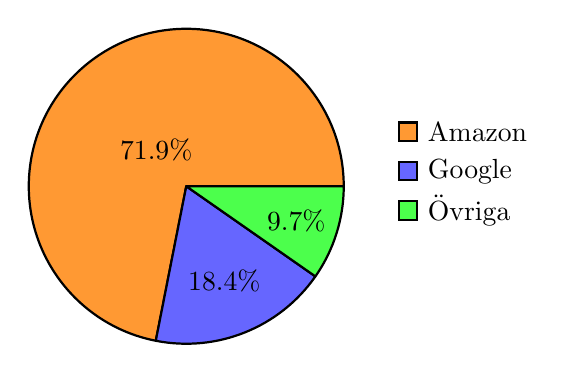
\begin{tikzpicture}
        \pie[text=legend, radius=2, color={orange!80, blue!60, green!70}]{71.9/ Amazon , 18.4/ Google , 9.7/ Övriga}
    \end{tikzpicture}
    \caption{\small Procentfördelning av enheterna i USA år 2017 \cite{voicebot}.}
    \label{fig:speaker_market_share}    
\end{figure}
Gemensamt för alla röst-produkter från Amazon och Google (men även Apple och Sonos) är att de är byggda proprietär programvara, källkoden är delvis eller helt stängd. En av nackdelen med stängd kod är att allmänheten saknar insyn i vad mjukvaran faktiskt gör och vilken data som enheten sparar. Detta oroar många potentiella konsumenter, sexton procent av de som inte äger en enhet uppger att oro kring integritet är en anledning till att de ännu inte köpt någon smart högtalare \cite{voicebot}. LITAR INTE PÅ FÖRETAGEN. SKRIV OM GOOGLE/NEST skandalen.

En fördel med en produkt som är baserad öppen mjukvara istället för proprietär sådan är också att användaren tillåts vara mer flexibel. Systemen kan ändras helt efter användarens behov och önskningar, just eftersom att kodbasen är fritt tillgänglig att modifiera. SKRIV OM FUNKTIONSNEDSÄTTNINGAR

\subsection{Syfte}
Syftet med detta praktiska gymnasiearbete är att bygga ett alternativ till de befintliga smarta högtalarna på den kommersiella marknaden. Frågeställningarna är därför: 
\begin{itemize}
\item Hur går man till väga för att bygga en smart högtalare med hjälp av öppen källkod?
\item Hur väl kan en egenbyggd enhet prestera?
\end{itemize}


\section{Metod och material} \label{metod}
Det viktigaste materialet som krävs för att konstruera en smart högtalare (med denna metod) och besvara frågeställningen är:
\begin{itemize}
\item Enkortsdatorn \textit{Raspberry Pi 3B+ } från The Raspberry Pi Foundation
\item Mikrofonkortet \textit{ReSpeaker 4-Mic Array for Raspberry Pi } från Seeed
\item Högtalaren \textit{Computer Speaker N90 }från Plexgear
\item Mjukvaruprojektet Mycroft som bearbetar, utför och besvarar användarens frågor och kommandon.
\end{itemize}
Utöver detta så behövs även några andra mindre ting för att genomföra arbetet. Däribland en flatkabel, koppartejp, ett minneskort till enkortsdator och PLA-filament eftersom det fysiska höljet produceras i 3D-skrivaren Ultimaker 3.



\section{Resultat}
\subsection{Elektronik}
Skriv om monterandet av komponenterna

\begin{figure}[H]
    \centering
    \caption{\small En av högtalarna nedmonterade}
    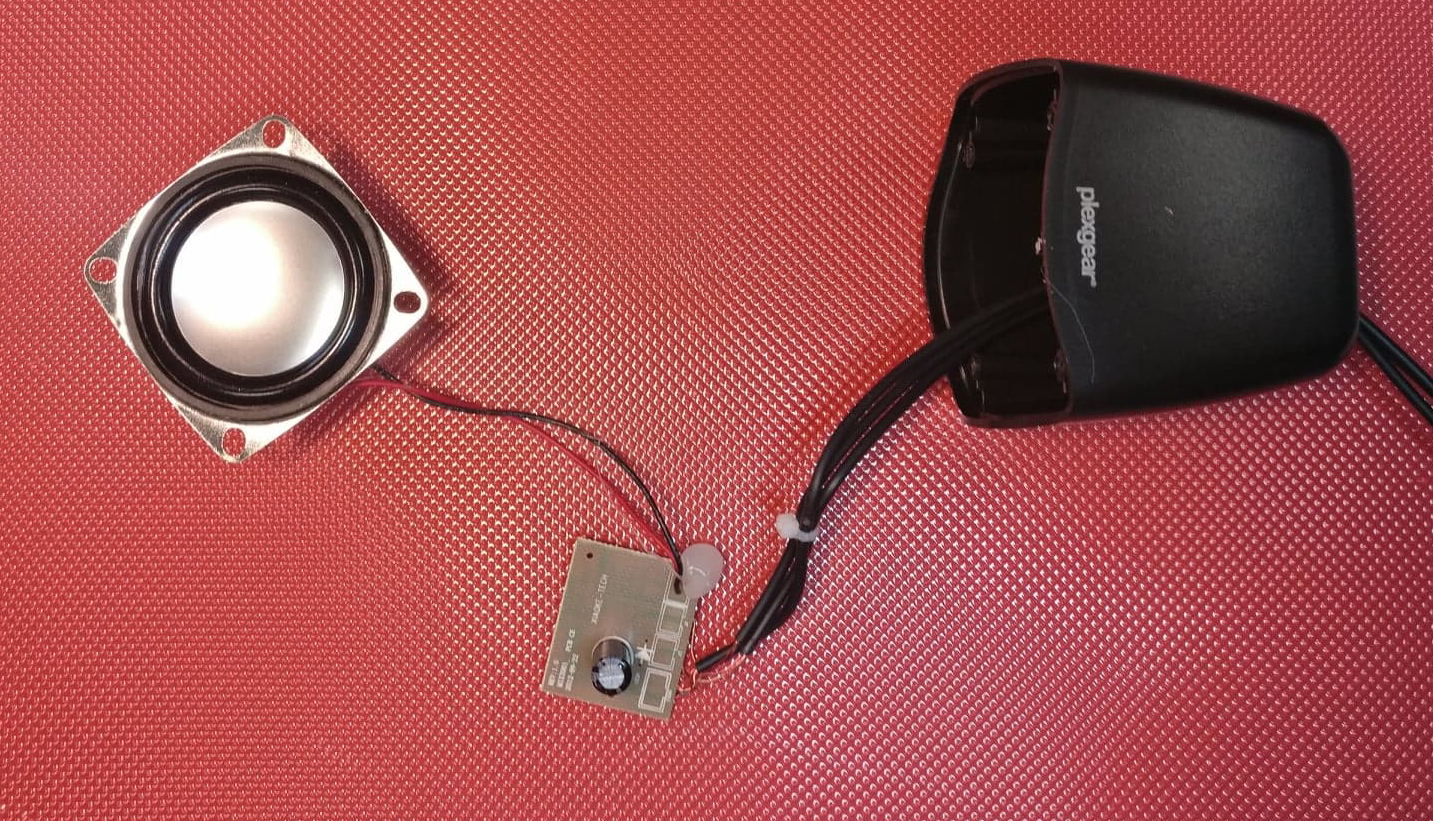
\includegraphics[width=12cm]{bilder/speaker_before_change.jpg}
\end{figure}
fiokopdfopsd
\begin{figure}[H]
    \centering
    \caption{\small Högtalarna tillsammans med den ombyggda, isolerade förstärkaren.}
    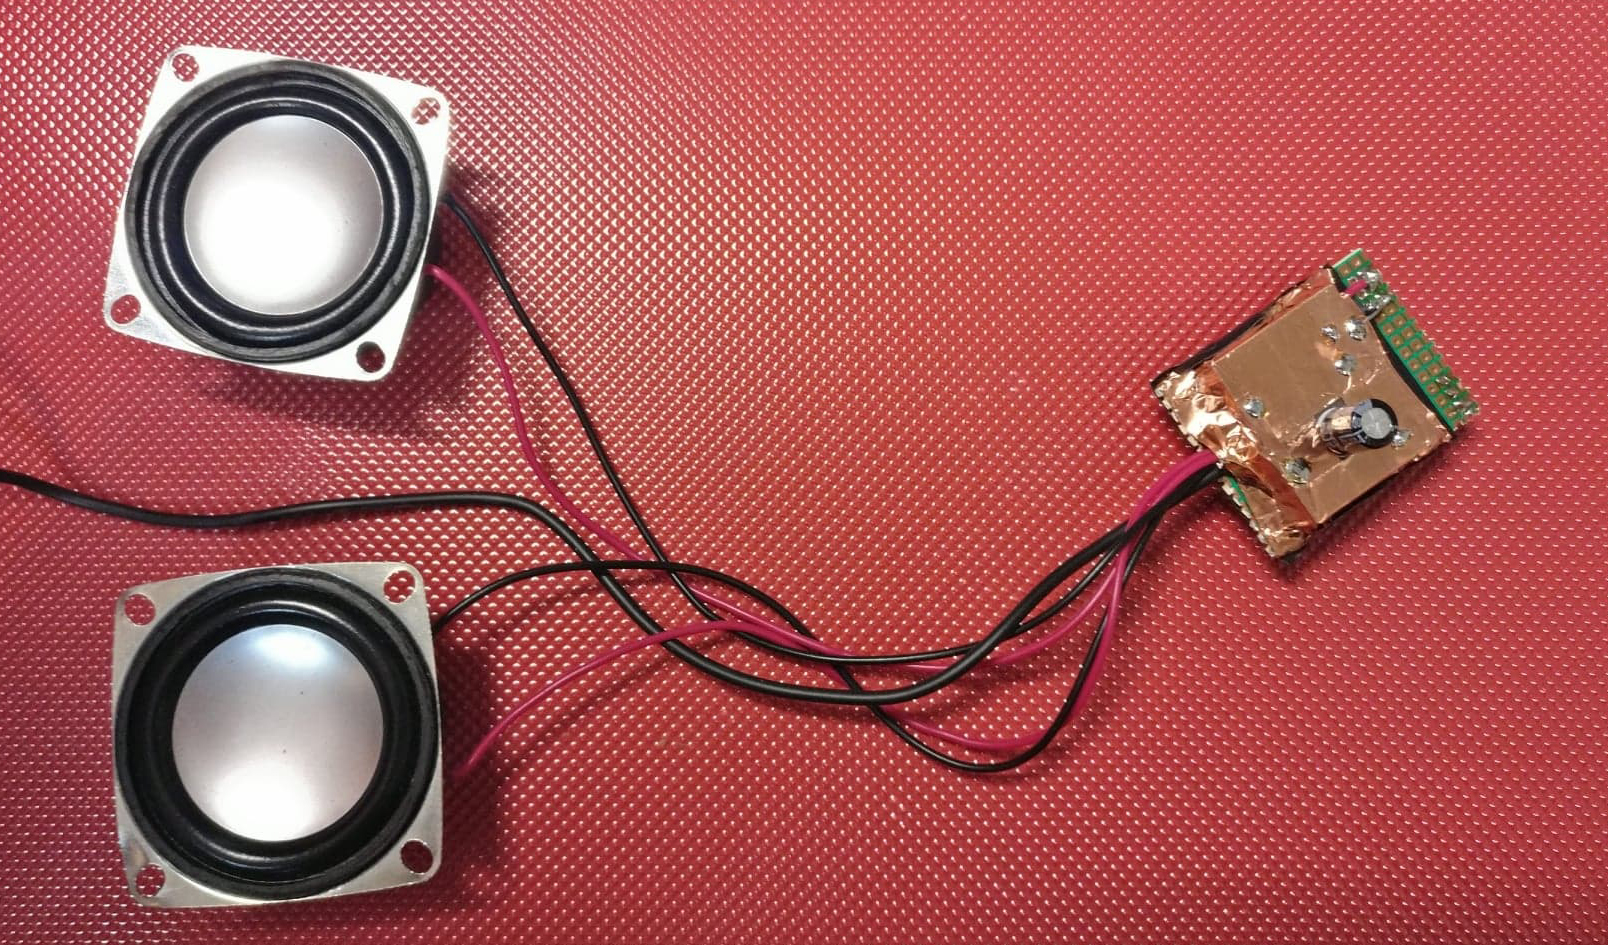
\includegraphics[width=12cm]{bilder/speakers_and_amplifier.jpg}
\end{figure}

\subsection{Mjukvara}
Som tidigare nämnt i avsnitt \ref{metod} så används mjukvaran Mycroft för att bearbeta, utföra och besvara alla kommandon och frågor som användaren ställer. 

För att enklast nyttja Mycroft-tjänsterna på en Raspberry Pi-dator så används Picroft – en fil med operativsystemet Raspbian Stretch Lite färdig\-paketerad med Mycroft \cite{picroft}. Äldre versioner av Picroft är dock inte kompatibel med Raspberry Pi modellen 3 B+.  Eftersom datormodellen i fråga är en del av detta projekt bör således den senaste versionen av Picroft (2018-9-12) användas för att mjukvaran ska fungera korrekt. För att faktiskt använda Picroft så hämtas en fil från internet och bränns sedan till ett micro-SD-kort. Minneskortet placeras i enkortsdatorn och enheten kan därefter startas.

Nästa steg i installationsprocessen är att ladda ner och installera drivrutiner till mikrofonen \cite{seeeds_documentation, reaspeker-installation}. Fabrikanten Seeeds egna drivrutiner laddas ner med hjälp av detta kommando:
\begin{minted}{bash}
git clone https://github.com/respeaker/seeed-voicecard.git
\end{minted}
Därefter installeras drivrutinerna och datorn startas om.
\begin{minted}{bash}
cd seeed-voicecard
sudo ./install.sh 4mic
sudo shutdown -r now
\end{minted}
I enkortsdatorns inbyggda konfigurationsmeny anges hålet för 3.5mm telepluggar som ljudutgång. 
\begin{minted}{bash}
sudo raspi-config
\end{minted}

För att få operativsystemet och Mycrofts röst-tjänster att korrekt använda sig av mikrofonen måste nu en asymmetrisk ljudenhet skapas i det inbyggda ljudsystemet ALSA. Detta åstadkoms genom att skapa filen \textit{~/.asoundrc} och placera följande rader kod i den:
\begin{minted}{bash}
pcm.!default {
    type asym
    playback.pcm "hw:0,0"
    capture.pcm "hw:1,0"
}
\end{minted}

Standardinställningarna som är angivna i den befintliga konfigurationsfilen \textit{/etc/asound.conf} måste även bytas ut till samma rader kod. Därefter startas datorn om. Efter omstart bör indikatorn för ljudnivå i Mycrofts användargränssnitt\footnote{Kommandot mycroft-cli-client används för att starta användargränssnittet} nu visa att mikrofonen fungerar korrekt. 
\\
SKRIV OM INTERNET-FIXEN, ändra setup wizard (eller var det någon annan fil) så att den pingar en vettig ip?
\\
Raspberry Pi-datorn har en röd lysdiod som lyser när strömmen är ansluten, detta stör rent estetiskt då det röda skenet kommer synas genom plasthöljet. Vi stänger av den genom att lägga till följande rad kod i filen \textit{/etc/rc.loca}l ovanför {\mintinline{latex}{exit 0}}: 
\begin{minted}{bash}
sudo sh -c "echo none > /sys/class/leds/led1/trigger"
\end{minted}

\subsection{Hölje och ihopmontering av enheten}
Höljet till den smarta högtalaren ritas i CAD-programmet Autodesk Inventor 2019. Höljet består av två delar, se figur \ref{fig:top-3d} och \ref{fig:bottom-3d}. I den nedre delen av högtalaren finns det skruvhål för att fästa enkortsdatorn och även hål dedikerade till ström, nätverks- och USB-ingångarna så att de alltid ska vara åtkomliga. Den övre delen av höljet har skruvhål för att fästa mikrofonkortet men även hål på sidan där högtalarna skall placeras. 
\begin{figure}[H]
    \centering
    \caption{\small Rendering av den övre halvan av höljet.}
    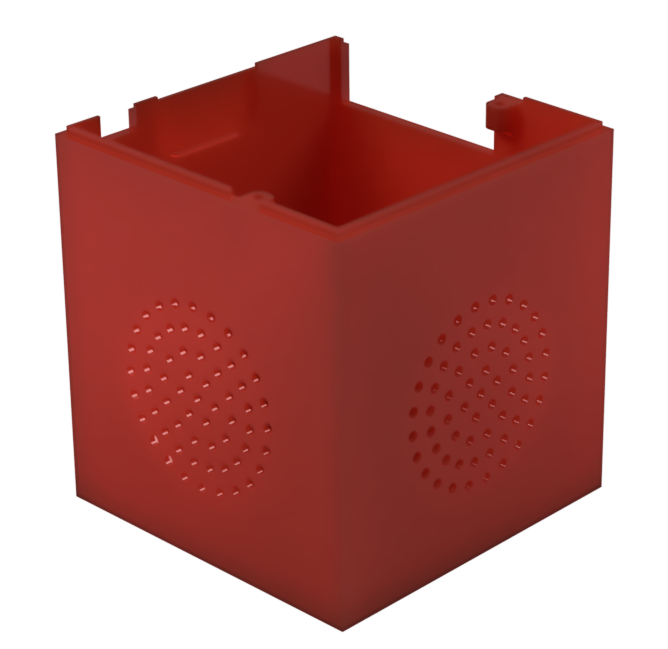
\includegraphics[width=9cm]{bilder/top_red.png}
    \label{fig:top-3d} 
\end{figure}

\begin{figure}[H]
    \centering
    \caption{\small Rendering av den nedre halvan av höljet.}
    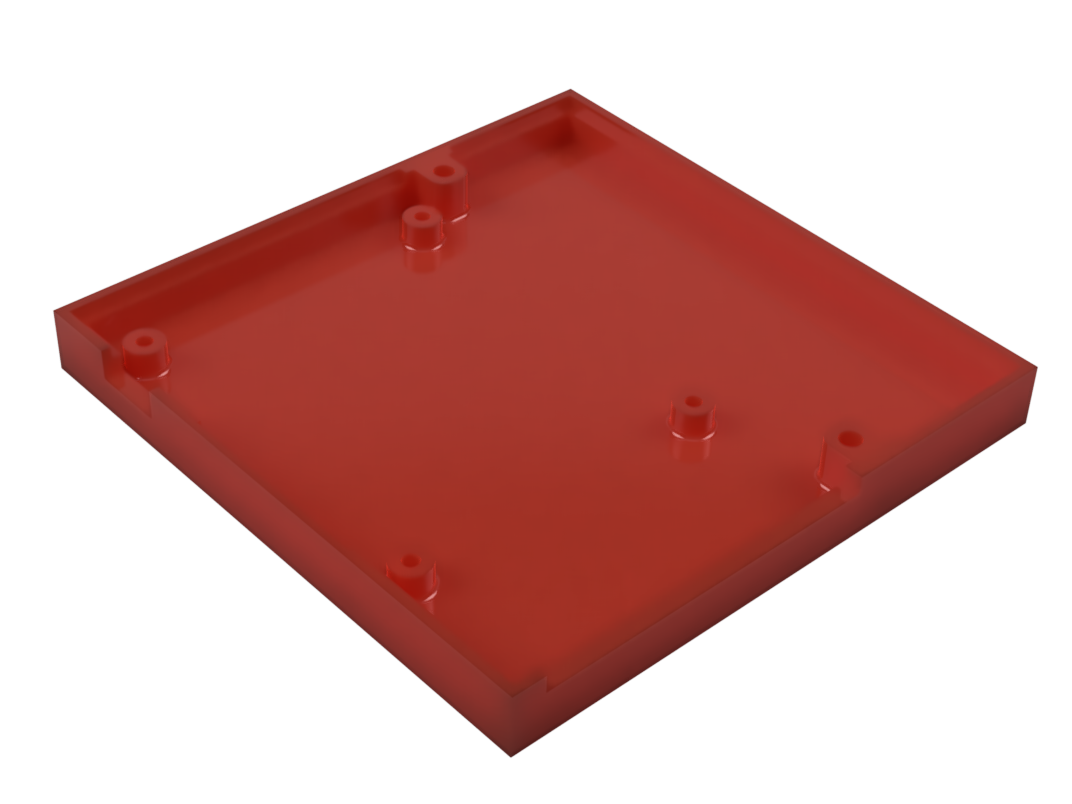
\includegraphics[width=9cm]{bilder/bottom_red.png}
    \label{fig:bottom-3d} 
\end{figure}

Efter de digitala 3D-filerna till höljet är färdigställda så produceras de två bitarna i 3D-skrivaren Ultimaker 3 med PLA-plast, i detta fallet röd sådan från skrivar\-tillverkaren själv. Det är även värt att notera att delarna är designade för att inte behövs några stödben när de skrivs ut.

När de båda delarna är utskrivna kan alla komponenter monteras i höljet. Mikrofonkortet och enkortsdatorn skruvas fast och ansluts till varandra med en flatkabel som även försörjer förstärkaren med ström. Högtalarna limmas fast på insidan, när dessa sitter fast kan slutligen höljets två delar skruvas samman och plastben klistras fast på undersidan.


\begin{figure}[H]
    \centering
    \caption{\small Bild av den färdiga prototypen.}
    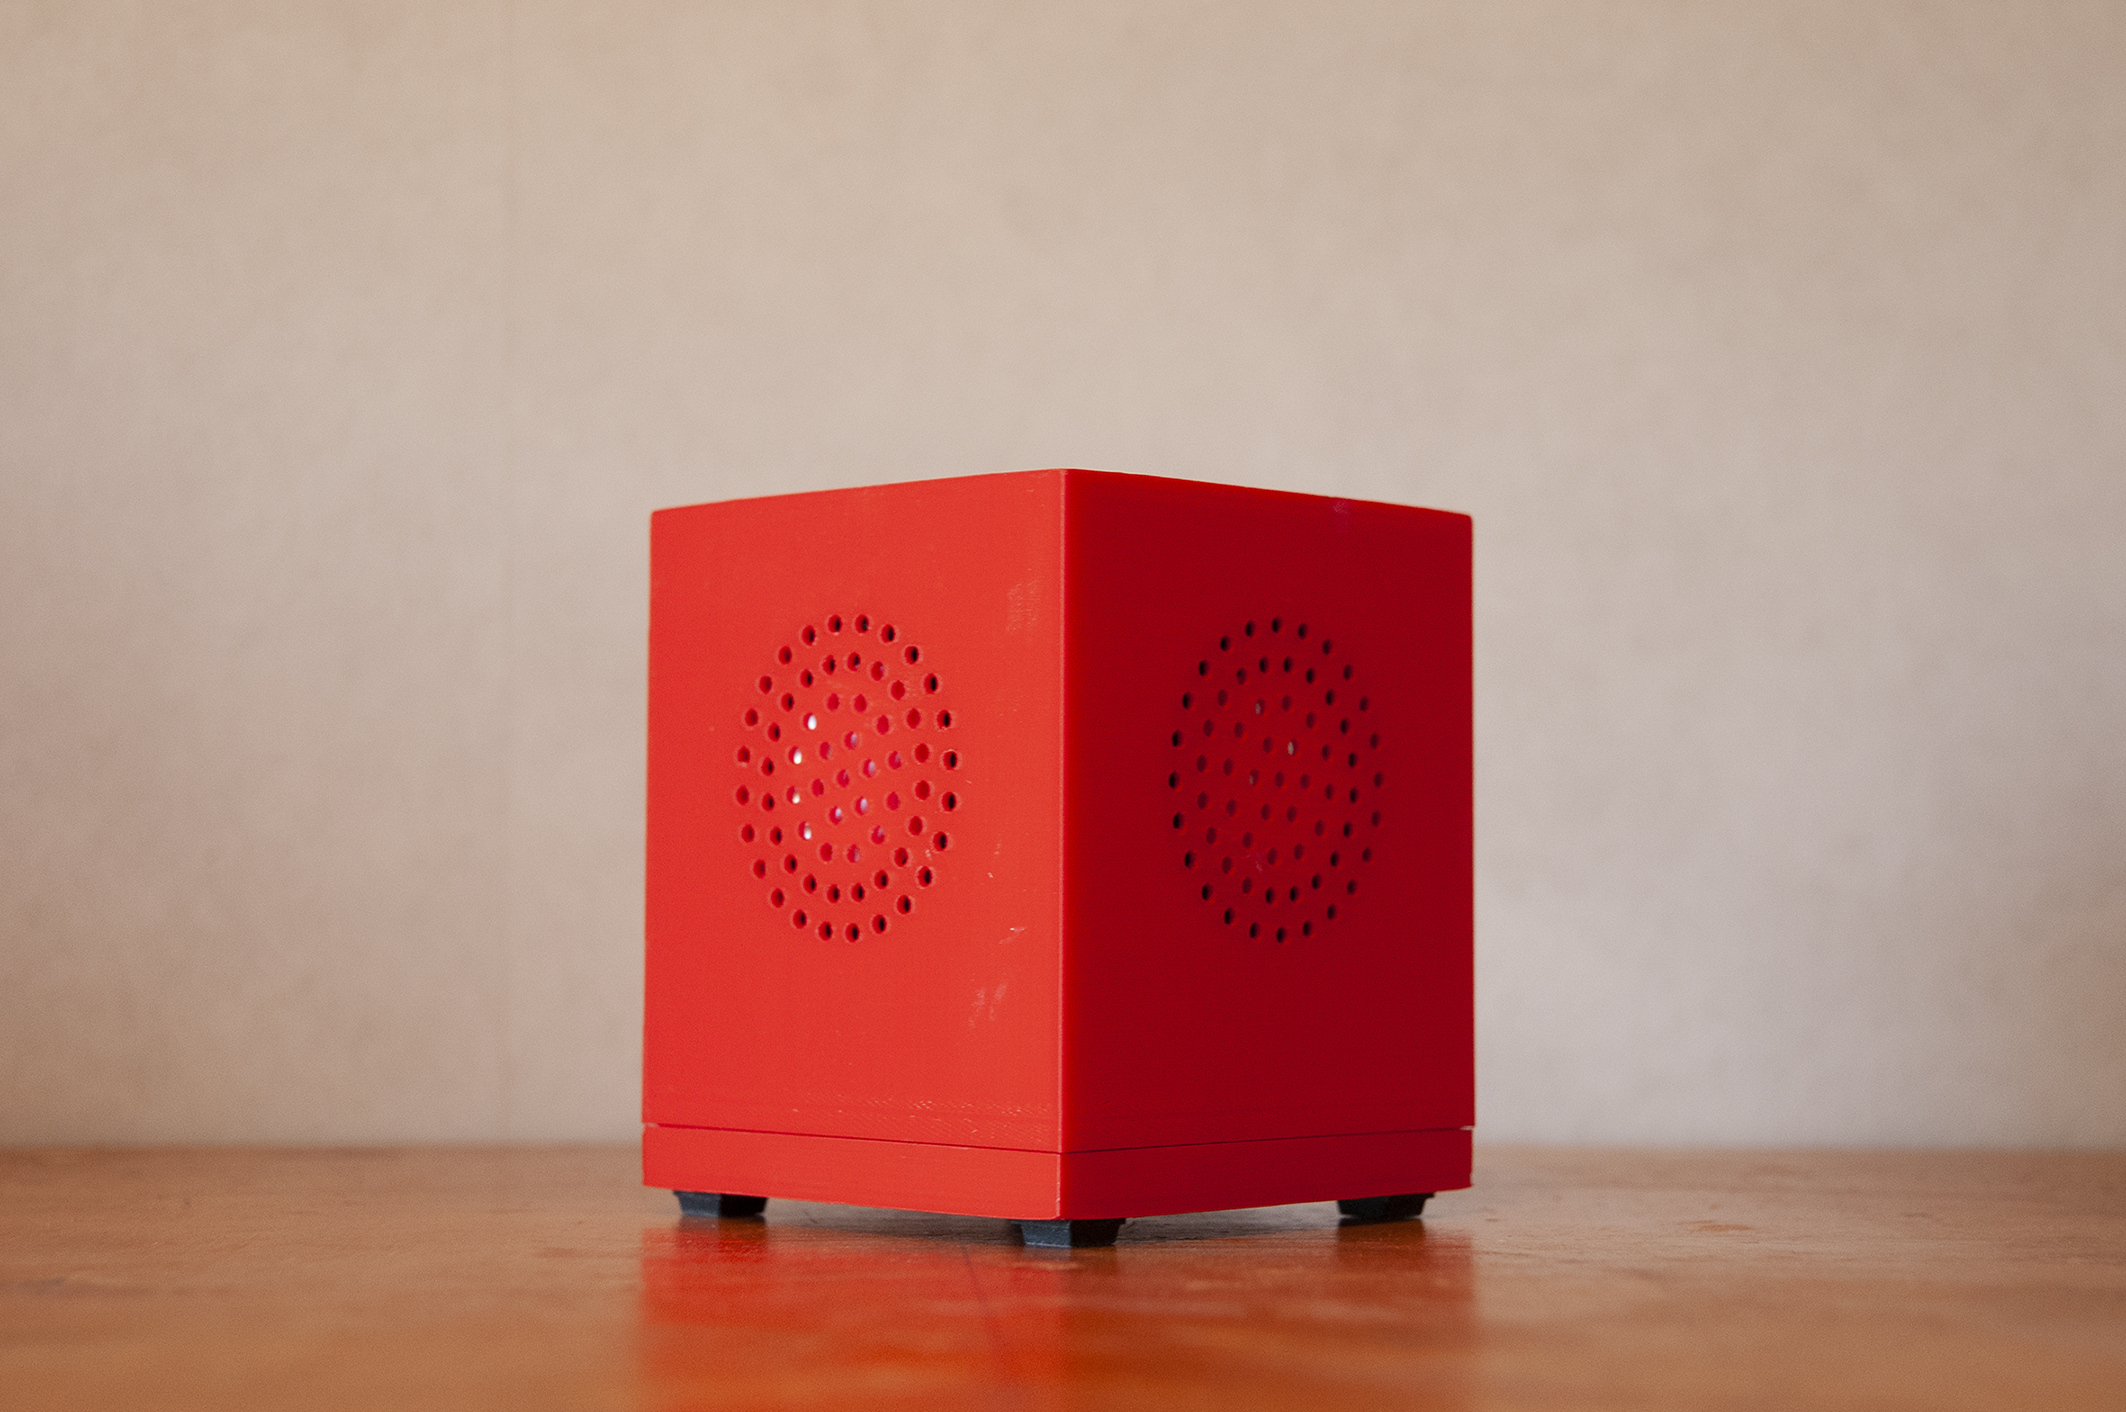
\includegraphics[width=14cm]{bilder/finale_unit_small.jpg}
    \label{fig:finale_unit} 
\end{figure}



\section{Diskussion}
Lång text om diskussion fposdk fposdk ofpsdk fpodsf kpsdo fkpodskf posdkf spodkf sopd

\subsection{Slutsats}
fsdjfdsp okf opsdkf psd fopkdsopf sdk fopsdk fsdkdopf kdsop

\section{Ta del av filerna}
Rapporten till detta gymnasiearbete är skriven i typsättningssystemet \LaTeX \ och alla filer som dokumentet utgörs av finns tillgängliga på hemsidan Github, se webbadressen nedan.  Rapporten är licensierat under \textit{Creative Common Attribution-NonCommercial-ShareAlike 4.0 International}. Detta innebär att det är tillåtet att fritt dela och modifiera rapporten under förutsättningarna att även den nya versionen bevarar samma licens, att det är i ett ickekommersiellt syfte samt att även jag nämns vid namn.

3D-filerna till höljet finns också att ladda ner på Github men även på plattformen Thingiverse. Dessa filer är dock licensierade under\textit{ Creative Common Attribution 4.0 International}. Jag måste alltså nämnas vid namn men i övrigt är du fri att göra vad du vill med filerna även när det rör sig om  kommersiella syften. \\

\noindent\textbf{Webbadresser}\\
\url{https://github.com/adelhult/gymnasiearbete}\\
\url{https://www.thingiverse.com/thing:3646712}


\newpage
\addcontentsline{toc}{section}{Referenser} 
\printbibliography

\end{document}